\chapter{Paper III:\@
  Overreact, an in silico lab:
  \linebreak automative quantum chemical microkinetic simulations
  for complex chemical reactions
 }%
\label{ch:paper3}

\citetext{Schneider2022}

\overreact is a software package for microkinetic modelling using data from
first-principles quantum chemical
calculations~\cite{Schneider2022,overreact2021zenodo}.
It is an improvement on a first attempt to build a
chemical chemical kinetics simulator that uses first-principles quantum
chemical calculations~\cite{pyrrole2019zenodo} (for a list of other software
contributions that have taken place during the course of the PhD, see~\cref{ch:all-works}).
Lessons learned from this first iteration, as well as the methodology
underlying \overreact, can be found in~\cref{sec:overreact-methods}.

HOW IS THE RESEARCH DESIGNED?\@

WHY IT IS DESIGNED THIS WAY?\@

WHAT DOES THE LITERATURE SAY ABOUT THIS?\@

IS THE LITERATURE WELL STABLISHED?\@
IS IT DIVIDED?\@

HOW DOES THE RESEARCH FIT THE BIGGER PICTURE?\@

HOW DOES THE RESEARCH CONTRIBUTE SOMETHING ORIGINAL?\@

HOW DOES THE METHODOLOGY OF PREVIOUS STUDIES HELP YOU DEVELOP YOUR OWN?\@

WHY IS THIS WORTH INVESTIGATING?\@
HOW IMPORTANT IS THIS?\@
HOW IS THIS ORIGINAL?\@

WHAT WERE MY RESEARCH AIMS?\@

WHAT IS THE SCOPE OF MY STUDY?\@
WHAT I COVERED AND DIDN'T COVER?\@

WHICH METHODS WERE USED?\@

\section{Background and motivation}

PRESENTATION OF THE WORK.\@

DESCRIPTION OF THE WORK.\@

OBJECTIVES OF THE WORK.\@

INTERPRETATION AND MEANING OF THE WORK.\@

MAIN FINDINGS.\@

RESULTS IN RELATION TO THE RESEARCH QUESTIONS.\@

Mecanismos foram validados com base na concordância relativa aos respectivos resultados experimentais~\cite{Kirby_1972,Jung_2005}.
A termoquímica relevante foi calculada à condição de temperatura e pressão ambientes (298.15~K e 1~atm).
Determinações de \emph{pKa} dos compostos estudados também foram realizadas com
relação ao ácido acético, de acordo com o esquema de
\citeauthor{Ding_2009}~\cite{Ding_2009} (\cref{sec:pka}).

Cálculos foram realizados com o programa Gaussian~09C.01~\cite{g09} e com o funcional da densidade
% PBE0~\cite{Perdew_1996,Perdew_1997,Ernzerhof_1999,Adamo_1999}
\emph{wB97XD}~\cite{Chai_2008a,Chai_2008b} (\cref{sec:funcionais}), que foi
utilizado em conjunto com funções de base de Pople de qualidade triplo-$\zeta$
com funções difusas e polarizações em todos os átomos
(\emph{6--311++G**}~\cite{Ditchfield_1971,Hehre_1972,Hariharan_1973,Hariharan_1974,Gordon_1980,Francl_1982,Clark_1983,Frisch_1984,Binning_1990,Blaudeau_1997,Rassolov_1998,Rassolov_2001},~\cref{sec:basis-functions}).
Todos os cálculos levaram em consideração efeitos de solvatação aquosa através
do uso do \emph{SMD}, desenvolvido por \citeauthor{Marenich_2009} (\cref{sec:implicit-solvation}).
De forma a se investigar o efeito da geometria do estado fundamental, uma
análise conformacional dos compostos foi empregada, usando o programa Open
Babel 2.4.1~\cite{O_Boyle_2011} com o \emph{PM7} (MOPAC2016~\cite{MOPAC},~\cref{sec:conformational-analysis}).

Estruturas eletrônicas dos compostos serão estudadas à luz dos \emph{NBO}
(\cref{sec:nbos}).
% , em particular para se correlacionar o efeito cinético da substituição
% \begin{enumerate*}[label=(\roman*)]
%   \item com eventuais flutuações de hibridização dos carbonos da ponte~\cite{Bent_1961} e
%   \item com a magnitude da repulsão estérica entre substituintes e grupos reativos.
% \end{enumerate*}
Para tanto será utilizado o programa NBO~5.9~\cite{NBO5.9} acoplado com o programa Gaussian~09C.01~\cite{g09}.

\section{Paper}

The publication can be read in full next.

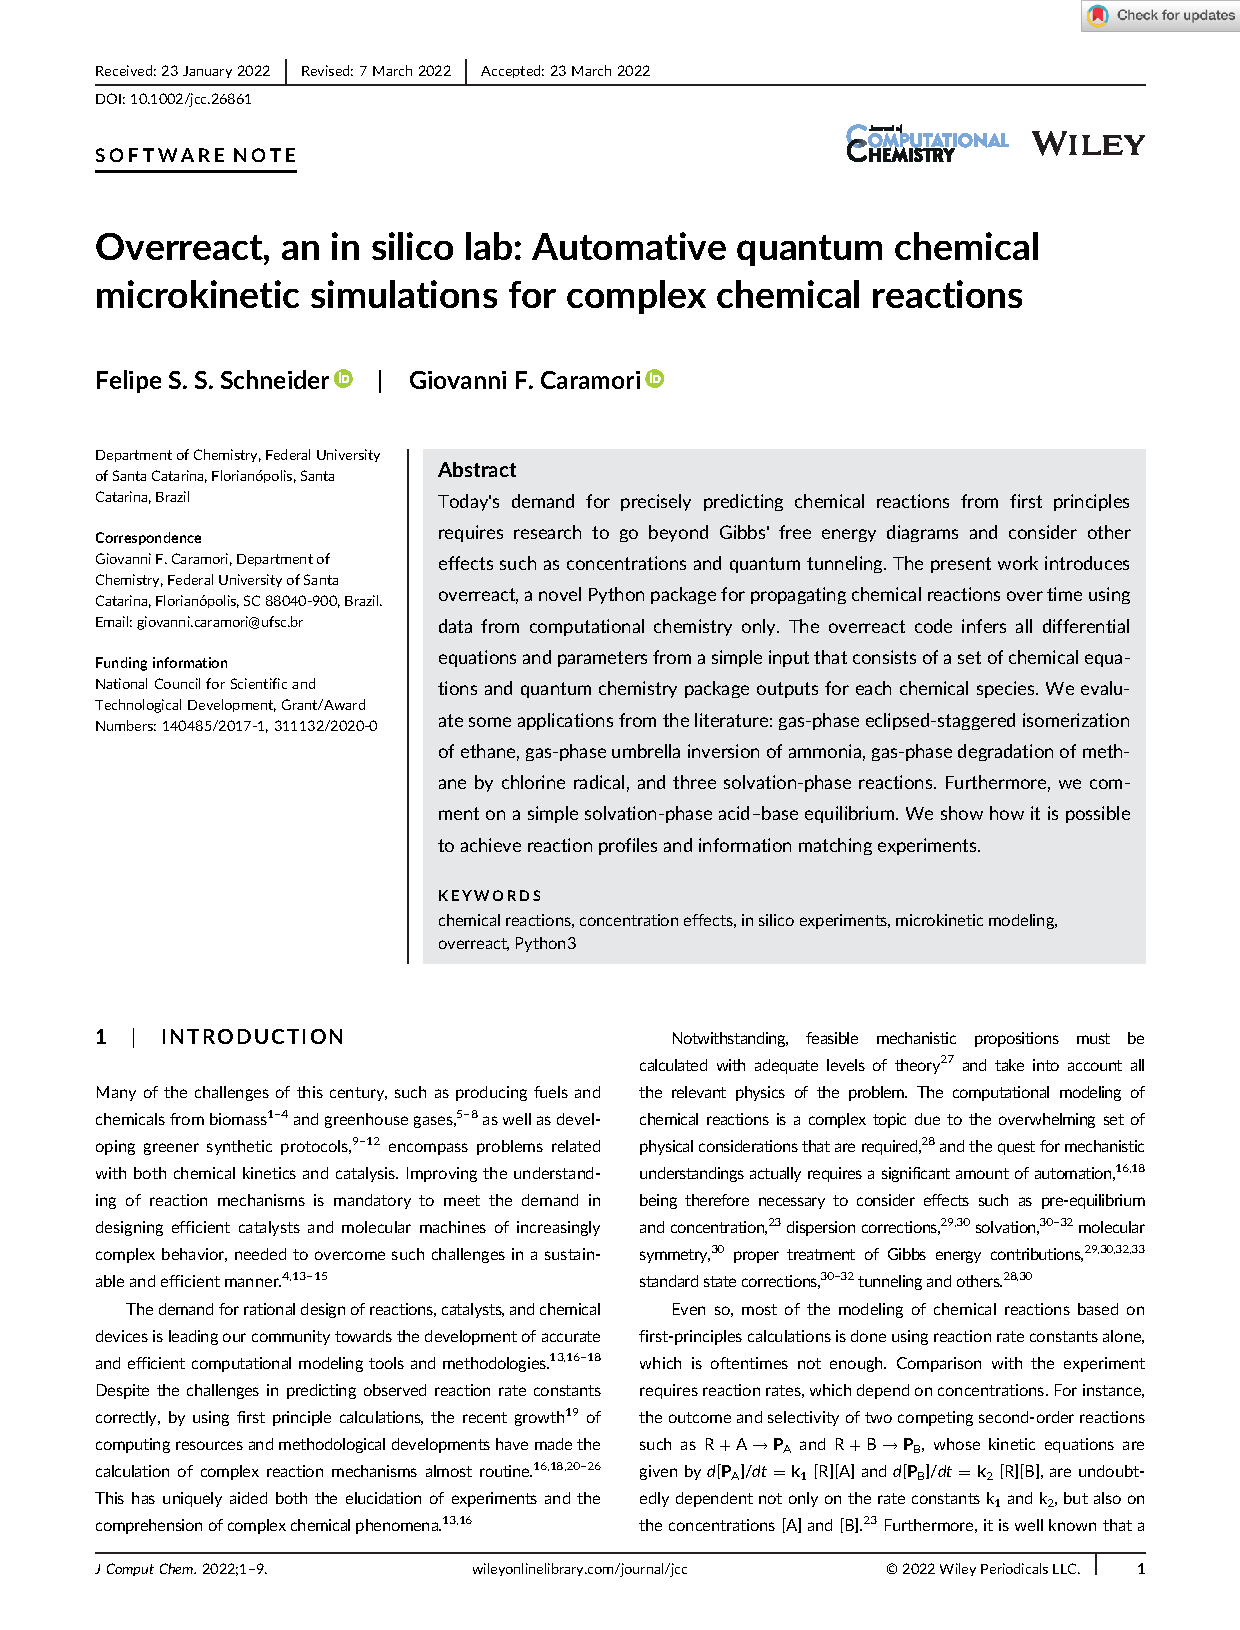
\includepdf[pages=-]{pubs/schneider2022-paper3.pdf}
